\section{Introduction}
Databases are susceptible to various forms of corruption, or \emph{dirtiness}, such as missing, incorrect, or inconsistent values.
Numerous surveys of industry have shown that dirty data are prevalent \cite{Gartner}, and there is now a growing industry around processing dirty data at scale \cite{fortunearticle}.
Analysts are increasingly deriving data from inherently error-prone processes such as extracting structured data from websites, synthesizing data from multiple networked sensors, and linking entities in disparate data sources.
As these data grow, new methodologies for scalable and reliable analysis in the presence of errors are required. 

Increasingly, modern data analysis pipelines involve Machine Learning for predictive models.
The endpoint of these pipelines can be any number of ``data products", such as recommender systems, spam detectors, and forecasting models, all of which can be very sensitive to data quality \cite{xiaofeature}.
When data error is systematic, or correlated with the data, errors can significantly bias predictions by a model.
For example, in a recommender system, we may find that all users from one region have a missing age attribute.
In this setting, discarding corrupted data or ignoring the problem can make predictions for the affected subpopulation untrustworthy.
A more sophisticated approach is to apply robust statistical methods, but these are designed to mitigate the effect of high-magnitude random outliers, and not compensate for systematic errors.

For some types of systematic error, we can apply data cleaning, which is an extensively studied field (see Rahm and Do \cite{rahm2000data} for a survey).
Instead of avoiding the problem, cleaning works by repairing (or approximately repairing) the corruption.
However, cleaning large data can be expensive, both computationally and in human effort, as an analyst has to program repairs for all errors manifest in the data \cite{kandel2012}.
In some applications, scripted data transformations may not be reliable necessitating the use of even costlier crowdsourcing techniques \cite{gokhale2014corleone,park2014crowdfill}.

An emerging solution to the growing costs of data cleaning is sampling \cite{wang1999sample} where the analyst cleans a small sample of data and can estimate the results of aggregate queries.Analysts can sample a large dataset, prototype changes on the sample, and evaluate whether these changes have the desired affect.
The case for sampling is analogous to arguments for Approximate Query Processing (AQP) \cite{DBLP:conf/eurosys/AgarwalMPMMS13}, where a timely approximate answer is more desirable than an exact slow answer.
Sampling provides a flexible tradeoff between cleaning cost and query result accuracy for aggregate queries, but the question we explore in this paper is how this tradeoff extends to Machine Learning. 

\begin{figure}[t]
\centering
 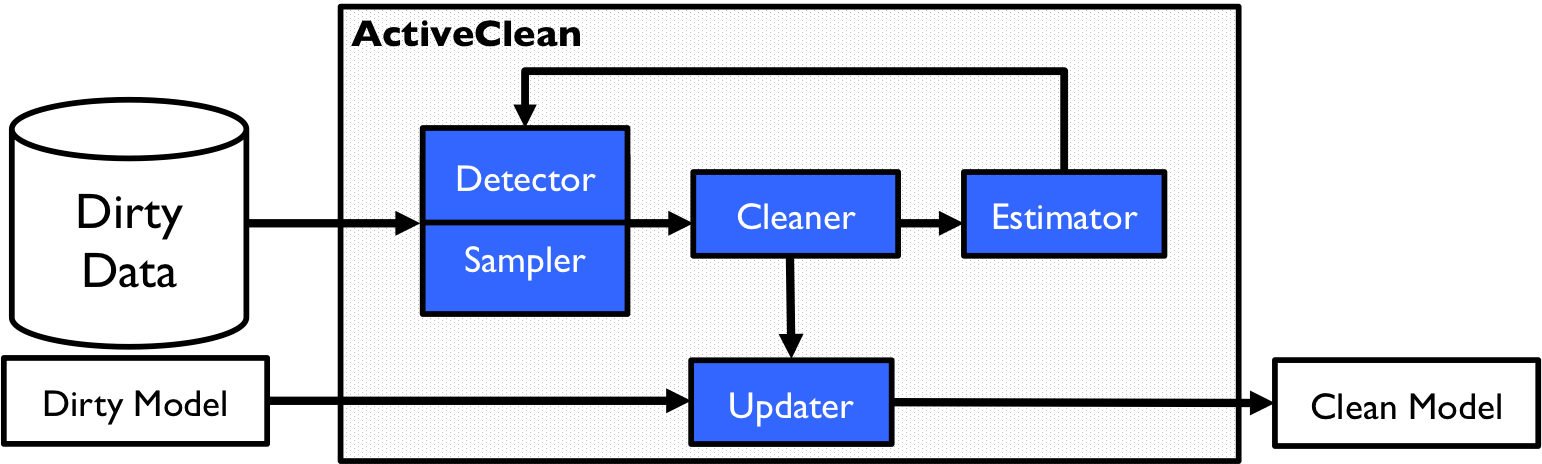
\includegraphics[width=0.6\columnwidth]{figs/arch.png}
 \caption{\sysfull (\sys) is an anytime framework from training models on dirty data. Expensive data transformations prior to model training are budgeted with a non-uniform sampling that prioritizes examples that are most likely to change the model.  \label{sys-arch}}
\end{figure}

Machine Learning is far more sensitive to sample size (training data) than aggregate queries.
However, there are a few observations that make this problem tractable.
Sampling is naturally part of large-scale Machine Learning, as stochastic optimization methods start at an arbitrary initialization and calculate updates by drawing training examples at random. 
Even with clean data, in very large datasets, it is well known that substantial progress is made in less than one epoch (i.e., a full pass through the entire dataset) \cite{bottou2012stochastic}.
In our setting, we do not have to start with an arbitrary initialization.
Errors often happen in batches, often tightly clustered, and affect a small number of features.
This means that a dirty model may be relatively ``close" to the clean model albeit with bias in a few features.
Hypothetically, if we had a clean dataset, and were to apply stochastic optimization using the dirty model as an initialization, we can get a highly accurate result with processing far less than an entire epoch.
This insight inspires the key idea of this paper, namely, that we can clean data as and when required by the optimization allowing us to clean far less than the entire dataset.

This integrated model training and data cleaning architecture leads to new optimization opportunities.
Since data cleaning adds a very significant cost to each model update, we can run pre-computations at each iteration to select which examples to clean because the additional overhead is offset by reductions in cleaning cost.
There is a growing consensus in Machine Learning research that all training data are not created equal and some data are more informative than others \cite{drineas2012fast, settles2010active}.
In Active Learning, we often sequentially select the most important points to label \cite{settles2010active}.
However, the key new challenge in data cleaning is that features and examples that may look unimportant in the dirty data may be important in the clean data and vice versa.
We partition data that we believe is clean from the dirty data, and estimate the effects of cleaning on the dirty data based on prior examples.
The resulting algorithm selects examples valuable to the clean model with higher probability and as an analyst cleans data we further guide the cleaning.

In this paper, we propose \sysfull (\sys), an anytime framework for training Machine Learning models with data cleaning.
In Figure \ref{sys-arch}, we illustrate our system architecture.
\sys supports a class of models called regularized-convex loss problems which includes linear regression, logistic regression, generalized linear models, and support vector machines.
We start with a model trained on the dirty data.
An \emph{error sampling} module selects a small sample of data from the corrupted dataset to clean.
We apply the repairs to this small sample with the \emph{error repair} module, and use an incremental optimization method (e.g., Gradient Descent) to update the dirty model.
Once we clean data, we maintain a running estimate of how cleaning impacts the model and feed that estimate back to adaptively set the sampling distribution.

In summary, our contributions are
\begin{itemize}[noitemsep]
\item We propose \sysfull which given dirty data, a convex loss model, and a time budget, returns a model trained with respect to the clean data.
\item \sysfull is implemented with an non-uniform importance sampling approach that prioritizes points in the clean model that are most informative, and we provide analysis to identify the key tradeoffs.
\item There are numerous database techniques that we apply to make this practical. We have to index dirty and clean data, amortize scan costs using shared cursors, and modify some data cleaning operations for correctness when applied to progressively increasing sample sizes.
\item We evaluate \sysfull on real and synthetic datasets to show that non-uniform sampling achieves improved performance in comparison to uniform sampling, and dirtiness-agnostic prioritization.
\end{itemize}








